% Created 2024-01-18 Thu 11:34
% Intended LaTeX compiler: xelatex
\documentclass[11pt]{article}
\usepackage{graphicx}
\usepackage{longtable}
\usepackage{wrapfig}
\usepackage{rotating}
\usepackage[normalem]{ulem}
\usepackage{amsmath}
\usepackage{amssymb}
\usepackage{capt-of}
\usepackage{hyperref}
\usepackage{minted}
\usepackage{xeCJK}
\setCJKmainfont{SimSong}
\setCJKmonofont{SimSong}
\let\oldsection\section
\renewcommand{\section}{\clearpage\oldsection}
\author{Chen Chen}
\date{\today}
\title{OCCT OCAF 学习笔记}
\hypersetup{
 pdfauthor={Chen Chen},
 pdftitle={OCCT OCAF 学习笔记},
 pdfkeywords={},
 pdfsubject={},
 pdfcreator={Emacs 29.1 (Org mode 9.7)}, 
 pdflang={English}}
\begin{document}

\maketitle
\tableofcontents

\section{Introduction}
\label{sec:org298c8bc}

\subsection{OCAF Module}
\label{sec:orgc59fadd}

\subsubsection{Overview}
\label{sec:org62d3e09}
Open CASCADE Technology (OCCT) 是一个开源的软件开发平台,用于三维 CAD、CAM、CAE 系统的开发。它提供了广泛的功能,涵盖了几何建模、图形可视化、数据交换和更多方面。

Open CASCADE Application Framework (OCAF) 是 OCCT 中的一个重要模块。OCAF 是一个应用程序框架,用于简化复杂工程图形应用程序的开发。它提供了一种有效的方式来组织、存储、检索和操作复杂的工程数据。OCAF 特别适合于需要处理复杂的装配结构、历史记录、参数化设计等场景的应用程序。
\subsubsection{OCAF 的主要功能}
\label{sec:orgee5b2a3}

\begin{itemize}
\item 数据管理
\begin{itemize}
\item OCAF 提供了一套工具来有效地管理和组织数据。
\item 这包括用于创建、管理和修改数据结构的 API
\end{itemize}
\item 历史记录和撤销/重做机制
\begin{itemize}
\item OCAF支持记录用户的操作历史,使得可以方便地实现撤销和重做功能。
\end{itemize}
\item 属性和关系管理
\begin{itemize}
\item OCAF允许开发者为数据元素定义属性(如颜色材料等),并管理数据元素间的关系。
\end{itemize}
\item 事务管理
\begin{itemize}
\item OCAF支持事务管理,这对于保证数据的一致性和完整性非常重要。
\end{itemize}
\item 扩展性
\begin{itemize}
\item OCAF设计灵活,易于扩展,开发者可以根据特定应用需求添加新的功能。
\end{itemize}
\end{itemize}

通过 OCAF,开发者可以更专注于应用的核心功能,而不是底层的数据管理和操作。
\subsubsection{OCAF 的主要 Packages}
\label{sec:orga124970}

下面列出了一些在 OCAF 中常用且重要的 packages:

\begin{itemize}
\item \textbf{TDF (Topological Data Framework)}
\begin{itemize}
\item 用于管理和存储拓扑数据的结构和信息。
\item TDF 提供了一个层次化的数据组织方式,通过 \texttt{Label}, \texttt{Attribute} 等来存储和管理数据
\end{itemize}
\item \textbf{TDocStd (Document Standard)}
\begin{itemize}
\item \texttt{TDocStd} 提供了创建、管理和保存文档的功能
\item 一个文档可以包含一个或多个 TDF 数据结构
\end{itemize}
\item \textbf{XCAF (eXtended CA Framework)}
\begin{itemize}
\item 用于更高级的 CAD 数据处理,如装配结构、颜色和层次信息。
\item XCAF 扩展了 OCAF 的功能,使其能够处理更复杂的 CAD 模型和数据
\end{itemize}
\item \textbf{TNaming (Naming)}
\begin{itemize}
\item 提供了一个命名服务,用于在模型中标识和追踪对象。
\item \texttt{TNaming} 使得在模型变更过程中可以保持对特定对象的引用。
\end{itemize}
\item \textbf{TPrsStd (Presentation Standard)}
\begin{itemize}
\item 用于关联数据模型和其图形表示
\item \texttt{TPrsStd} 允许开发者定义如何将模型数据转换为可视化的图形表示
\end{itemize}
\item \textbf{TDataStd (Data Standard)}
\begin{itemize}
\item 包含了一系列的 Attribute 类型,如字符串、整数、实数、枚举类型等。
\item TDataStd 提供了基础的数据类型,用于存储和处理常规属性。
\end{itemize}
\item \textbf{AppStdL (Application Standard Library)}
\begin{itemize}
\item 提供了一组标准的应用程序功能和服务,如历史管理、撤销/重做机制等。
\end{itemize}
\item \textbf{BinTObj}
\begin{itemize}
\item 用于持久化存储和加载 OCAF 对象的包。
\item 支持二进制格式,适用于大型数据集。
\end{itemize}
\item \textbf{XmlTObj}
\begin{itemize}
\item 类似于 BinTObj,但用于处理基于 XML 的持久化存储和加载。
\end{itemize}
\end{itemize}
\subsection{TDF Package}
\label{sec:orgec60fe2}

\subsubsection{Overview}
\label{sec:orgcde6654}

TDF (Topology Data Framework) 是 OCAF 的核心组件,用于管理和组织复杂的工程数据(其中拓扑数据是几何建模的基础)。TDF 提供了一个结构化的方式来存储和操作与拓扑相关的信息,如点、线、面、实体等几何元素及其之间的关系。
\subsubsection{TDF 的功能与职责}
\label{sec:orga5179ab}

\begin{itemize}
\item 数据组织

TDF 提供了一种层次化的数据结构,使得对复杂拓扑数据的管理和访问更加直观灵活。

\item 事务管理

通过 TDF,可以实现对拓扑数据的事务管理,支持撤销/重做操作,保证数据一致性。

\item 属性管理

TDF 允许为拓扑元素附加属性(颜色材料等),并管理这些属性。

\item 关系管理

TDF 支持管理拓扑元素之间的关系,如约束、连接等。

\item 版本控制

TDF 支持数据的版本控制,这对于跟踪数据的历史变更非常有用。

\item 灵活性和扩展性

TDF 设计灵活,易于扩展,可以根据特定的应用需求进行定制。
\end{itemize}
\subsubsection{TDF 的核心类}
\label{sec:org19aa7e5}

\begin{itemize}
\item \texttt{TDF\_Label} class 代表数据结构中的一个节点,可包含多个 sub-Labels 和 Attribute。
\item \texttt{TDF\_Attribute} class 附加在 Label 上的数据单元,用于存储特定类型的信息,如几何数据、颜色、文本等。
\item \texttt{TDF\_Data} class 代表整个数据集合,包含一个或多个 \texttt{TDF\_Label} 树
\item \texttt{TDF\_TagSource} class 用于自动生成唯一的 Tag (标签号)。
\item \texttt{TDF\_RelocationTable} class 在数据复制和粘贴操作中使用,管理 Label 和 Attribute 之间的关系映射。
\end{itemize}
\subsection{TDocStd Package}
\label{sec:org003da65}

\subsubsection{Overview}
\label{sec:org30c665f}
\texttt{TDocStd} 主要用于处理和管理文档(Document),这些文档用于存储和组织复杂的 CAD 数据结构。一个文档通常代表一个工程项目或一个 CAD 模型,它包含了所有相关的数据和信息。 \texttt{TDocStd} 提供了一套工具和接口来创建、管理和存储这些文档。
\subsubsection{TDocStd 的功能与职责}
\label{sec:org444799c}

\begin{itemize}
\item 文档管理

\texttt{TDocStd} 提供了创建和管理文档的基本机制。文档可以包含多种类型的数据,如几何形状、装配信息、属性等。

\item 文档结构

文档中的数据通过 OCAF 的 \texttt{TDF\_Label} 结构进行组织。每个文档都有一个 root Label, 从 root Label 开始可以创建一个层次化的数据结构。

\item 事务管理

\texttt{TDocStd} 支持事务管理,允许用户对文档进行修改操作,同时支持 Undo/Redo 功能。这对于保持数据的一致性和完整性至关重要。

\item 存储和加载

\texttt{TDocStd} 提供了将文档保存到文件系统和从文件系统加载文档的功能。支持多种格式,包括自定义格式。

\item 版本控制

文档可以支持版本控制,允许跟踪文档的历史变更。

\item 扩展性

\texttt{TDocStd} 的设计允许开发者根据需要扩展和定制文档的功能,以适应特定的应用需求。
\end{itemize}
\subsubsection{TDocStd 与 TDF package 的关系}
\label{sec:org3915a23}

\begin{itemize}
\item \texttt{TDocStd} 依赖于 \texttt{TDF} 来组织文档内的数据。

每个 \texttt{TDocStd\_Document} 包含一个根 \texttt{TDF\_Label}, 这个 root label 是文档所有数据的起点。通过 root label, 可以访问和操作文档中的所有数据。

\item 在 TDF 基础上,TDocStd 提供了文档级别的管理,如创建/保存/加载文档、事务处理(Undo/Redo)等。
\end{itemize}
\subsubsection{TDocStd 的核心类}
\label{sec:orgbf4d7d5}

\begin{itemize}
\item \texttt{TDocStd\_Document} class 代表一个文档,是管理和组织 CAD 数据的主要实体。
\item \texttt{TDocStd\_Application} class 处理文档的创建、加载和保存,管理文档集合。
\item \texttt{TDocStd\_Owner} class 作为文档所有者的角色,管理文档的状态和事务。
\end{itemize}
\subsection{XCAF Package (属于 DataExchange Module)}
\label{sec:org94d6a4c}

\subsubsection{Overview}
\label{sec:org56144a3}

XCAF (eXtended CA Framework) 用于处理更高级别的 CAD 数据,尤其是那些涉及到复杂装配结构的数据。XCAF 提供了一些列工具和接口,用于管理和操作包括颜色、材料、元数据、层级关系等在内的复杂 CAD 模型数据。
\subsubsection{XCAF 主要功能与职责}
\label{sec:orgbc0ada2}

\begin{itemize}
\item 复杂装配结构管理

XCAF 提供了工具来创建和管理复杂的 CAD 装配结构,包括定义装配体、子装配体和零件之间的层级关系。

\item 颜色和图层管理

支持为模型的不同部分指定颜色和图层,帮助改善模型的可视化和组织。

\item 高级属性管理

XCAF 允许为模型元素添加和管理高级属性,如材料属性、PMI(产品和制造信息)、注释和元数据。

\item 形状标识和追踪

提供工具来唯一标识和追踪模型中的形状,尤其在模型的变更或更新过程中,保持对特定形状的引用。

\item 数据交换支持

支持与其他 CAD 系统间的数据交换,特别是在处理 STEP 和 IGES 文件格式时,能够导入和导出中配信息和属性。

\item 扩展性和定制

XCAF 设计灵活,可以根据特定应用需求进行扩展和定制。
\end{itemize}
\subsubsection{XCAF 的核心类}
\label{sec:org6b0d519}

\begin{itemize}
\item \texttt{XCAFDoc\_ShapeTool} class 用于管理装配结构和形状。
\item \texttt{XCAFDoc\_ColorTool} class 管理颜色属性
\item \texttt{XCAFDoc\_LayerTool} class 管理图层属性
\item \texttt{XCAFDoc\_MaterialTool} class 管理材料属性
\item \texttt{XCAFDoc\_DatumTool}, \texttt{XCAFDoc\_DimTolTool} classes 管理标注和公差。
\item \texttt{XCAFDoc\_AreaStyleTool} class 管理区域样式
\end{itemize}
\subsection{TNaming package}
\label{sec:org3419c8b}

\subsubsection{Overview}
\label{sec:org1b53478}

\texttt{TNaming} 提供了命名服务,以便在复杂的 CAD 模型和数据结构中标识和追踪对象。这对于在模型变更过程中保持对特定对象的引用非常重要。
\subsubsection{TNaming 的主要功能与职责}
\label{sec:orgd8971bd}

\begin{itemize}
\item 对象标识和追踪

\texttt{TNaming} 允许用户为模型中的对象(如形状、特征等)赋予唯一的名称,从而在整个模型的生命周期中追踪和引用这些对象。

\item 历史追踪

支持记录和跟踪对象随时间的变化。这使得即使在模型被修改或更新后,也能够识别和访问原始对象。

\item 版本控制

\texttt{TNaming} 提供了一种机制来处理模型中对象的版本控制,保证在多次修改和迭代中对象的一致性。

\item 复杂操作支持

对于复杂的操作(如布尔运算、分割、修剪等), \texttt{TNaming} 能够帮助保持对影响的对象的引用,确保数据的准确性和完整性。

\item 与 TDF 协同工作

\texttt{TNaming} 与 \texttt{TDF} 紧密协作,利用 \texttt{TDF\_Label} 和 \texttt{TDF\_Attribute} 来存储和管理命名信息。

\item 撤销/重做机制支持

支持与 OCAF 的撤销/重做机制结合使用,确保在运行这些操作时保持命名信息的一致性。
\end{itemize}
\subsubsection{TNaming 的核心类}
\label{sec:org2d11256}

\begin{itemize}
\item \texttt{TNaming\_NamedShape} class 用于关联形状(Shape)与名称,实现形状的命名和追踪。
\item \texttt{TNaming\_Builder} class 用于构建和修改命名关系
\item \texttt{TNaming\_Tool} class 提供一系列静态方法来操作和查询命名信息
\item \texttt{TNaming\_Naming} class 存储和管理命名操作的历史记录。
\item \texttt{TNaming\_NamingTool} class 提供用于执行复杂命名操作的高级方法
\end{itemize}
\subsection{TPrsStd package}
\label{sec:org93c06e5}

\subsubsection{Overview}
\label{sec:org18af333}

\texttt{TPrsStd} package 用于将工程数据(如存储在 OCAF 文档中的数据)与其图形表示相关联。它为开发者提供了一系列工具和接口,以便在图形界面中展示和交互复杂的工程模型。
\subsubsection{TPrsStd 主要功能与职责}
\label{sec:orgdecf585}

\begin{itemize}
\item 图形表示管理

\texttt{TPrsStd} 使得开发者可以将工程数据(如形状、属性等)与其在图形用户界面中的视觉表示相关联。这包括形状的渲染、颜色、纹理等。

\item 交互和选择支持

提供了工具来支持用户与图形表示的交互,包括选择、高亮显示和编辑操作。

\item 属性与视觉同步

确保工程数据的更改能够实时反映在图形表示上,例如当形状发生变化时,其视觉表示也会相应更新。

\item 高级显示功能

支持高级的显示功能,如透明度、阴影和纹理映射,使得工程模型的视觉表示更加逼真和详细。

\item 自定义显示属性

允许开发者定义自己的显示属性和表示方式,以满足特定应用的需求。

\item 与 OCAF 结合使用

\texttt{TPrsStd} 与 OCAF的其他组件(如 \texttt{TDF\_Label}, \texttt{TDF\_Attribute})紧密集成,使得开发者可以方便地管理和同步数据与其图形表示。

\item 支持多种渲染引擎

可以与 OCCT 提供的不同渲染引擎(如OpenGL)协同工作,提供高质量的图形输出。
\end{itemize}
\subsubsection{TPrsStd 的核心类}
\label{sec:orgc3494ad}

\begin{itemize}
\item \texttt{TPrsStd\_AISPresentation} class 用于管理工程数据的图形表示,如形状在图形界面中的显示。
\item \texttt{TPrsStd\_AISViewer} class 提供一个视图环境,用于显示和管理多个图形表示。
\item \texttt{TPrsStd\_Presentation} class 作为数据和其图形表示之间的桥梁。
\item \texttt{TPrsStd\_Driver} class 为具体的数据类型提供图形表示的生成和更新逻辑。
\end{itemize}
\subsection{TDataStd package}
\label{sec:orgb3628d8}

\subsubsection{Overview}
\label{sec:orgf182336}

\texttt{TDataStd} 主要提供了一系列标准的数据属性(Attributes),这些属性可以附加到 OCAF 文档中的 Labels 上,用于存储和管理各种类型的数据。
\subsubsection{TDataStd 主要功能与职责}
\label{sec:orgd581450}

\begin{itemize}
\item 基本数据类型的管理

\texttt{TDataStd} 提供了用于存储基本数据类型(如字符串、整数、实数、布尔值等)的属性。这些属性用于存储和检索与标签相关联的基本信息。

\item 集合和列表的管理

提供了管理数据集合(如数组、列表)的属性,用于存储多个数据项。

\item 命名和标识符管理

支持为标签分配名称和标识符,方便数据的识别与引用。

\item 枚举和状态管理

提供了用于管理枚举值和状态的属性,可以用于表示有限的选择集或状态机。

\item 文档的元数据管理

支持存储文档级别的元数据,如作者、版本信息、注释等。

\item 与 \texttt{TDF\_Label} 结合使用

\texttt{TDataStd} 的属性与 \texttt{TDF\_Label} 紧密集成,使得数据可以方便地附加到标签上,并在 OCAF 文档的层次化结构中进行管理。
\end{itemize}
\subsubsection{TDataStd 的核心类}
\label{sec:orgc6088a9}

\begin{itemize}
\item \texttt{TDataStd\_Integer} 用于存储和管理整数值
\item \texttt{TDataStd\_Real} 用于存储和管理实数值
\item \texttt{TDataStd\_String} 用于存储和管理字符串
\item \texttt{TDataStd\_UAttribute} 作为用户自定义数据的基类,可以派生出用于存储特定类型数据的类。
\item \texttt{TDataStd\_Name} 用于存储和管理对象的名称
\item \texttt{TDataStd\_Boolean} 用于存储和管理布尔值
\item \texttt{TDataStd\_Enum} 用于存储和管理枚举值
\end{itemize}
\subsection{BinTObj package}
\label{sec:org7b716e5}

\subsection{XmlTObj packages}
\label{sec:org4caad02}
\section{开发环境搭建}
\label{sec:org96ffdec}

\subsection{Ubuntu 环境下编译与配置 OCCT 开发环境}
\label{sec:org39b26d3}

\begin{enumerate}
\item 安装依赖

首先安装所有必要的依赖包,通常包括编译器、构建工具和其他库等。

\begin{minted}[]{bash}
  sudo apt-get update
  sudo apt-get install build-essential cmake\
      git libfreetype6-dev libfontconfig1-dev\
      libx11-dev libxext-dev libxt-dev libxmu-dev\
      libgl1-mesa-dev tcl-dev tk-dev
\end{minted}

\item 获取 OCCT 源代码

你可以从 \href{https://dev.opencascade.org/release}{OpenCASCADE} 官网或 \href{https://github.com/Open-Cascade-SAS/OCCT}{GitHub} 上的仓库获取源代码。

\begin{minted}[]{bash}
  mkdir ~/geom
  cd ~/geom
  git clone https://github.com/Open-Cascade-SAS/OCCT.git
\end{minted}

\item 编译与安装 OCCT

\begin{itemize}
\item 使用 CMake 来配置构建系统,创建一个构建目录,在其中运行 cmake

\begin{minted}[]{bash}
    mkdir occt-build
    mkdir occt-install
    cd occt-build
    cmake ../OCCT -DCMAKE_INSTALL_PREFIX=./occt-install
\end{minted}

\item 编译 OCCT 库: \texttt{make -j\$(nproc)}
\item 安装 OCCT 库: \texttt{sudo make install}
\end{itemize}

\item 配置环境变量

设置环境变量以使编译器和连接器能够找到 OCCT 的头文件和共享库。在 \texttt{\textasciitilde{}/.bashrc} 或 \texttt{\textasciitilde{}/.profile} 中添加如下内容

\begin{minted}[]{shell}
  export CASROOT=~/geom/occt-install
  export LD_LIBRARY_PATH=$CASROOT/lib:$LD_LIBRARY_PATH
\end{minted}
\end{enumerate}
\subsection{编写简单的 OCCT 程序}
\label{sec:org8f689df}

OCCT 安装完成后,我们可以通过编译运行一个简单的 OCCT 示例程序来验证安装。

新建项目目录 \texttt{\textasciitilde{}/hello-occt/}, 新建项目文件 \texttt{CMakeLists.txt} 和 \texttt{main.cpp}. \texttt{CMakeLists.txt} 的内容如下:

\begin{minted}[]{cmake}
cmake_minimum_required(VERSION 3.10)
project(hello-occt)

set(CMAKE_CXX_STANDARD 17)
set(CMAKE_CXX_STANDARD_REQUIRED ON)

find_package(OpenCASCADE REQUIRED)

include_directories(${OpenCASCADE_INCLUDE_DIR})

set(SOURCES main.cpp)
add_executable(${CMAKE_PROJECT_NAME} ${SOURCES})

target_link_libraries(${CMAKE_PROJECT_NAME} ${OpenCASCADE_LIBRARIES})
\end{minted}

\begin{itemize}
\item \texttt{project(hello-occt)} 设置项目的名称
\item \texttt{set(CMAKE\_CXX\_STANDARD 17)} 指定 C++ 标准
\item \texttt{find\_package(OpenCASCADE REQUIRED)} 查找并加载 OCCT 库
\item \texttt{include\_directories(\$\{OpenCASCADE\_INCLUDE\_DIR\})} 添加 OCCT 头文件的路径
\item \texttt{set(SOURCES ...)} 定义了项目的源文件
\item \texttt{add\_executable(\$\{CMAKE\_PROJECT\_NAME\} \$\{SOURCES\})} 创建一个可执行文件
\item \texttt{target\_link\_libraries(\$\{CMAKE\_PROJECT\_NAME\} \$\{OpenCASCADE\_LIBRARIES\})} 链接 OCCT 库
\end{itemize}

下面的验证程序,创建一个简单的长方体,然后获取其 Topo Shape。源代码文件 \texttt{main.cpp} 如下

\begin{minted}[]{cpp}
#include <iostream>
#include <BRepPrimAPI_MakeBox.hxx>
#include <TopoDS_Shape.hxx>

int main() {
  BRepPrimAPI_MakeBox box(1., 2., 3.);
  const TopoDS_Shape& shape = box.Shape();
  std::cout << "Hello OCCT" << std::endl;
  return 0;
}
\end{minted}

按照如下的方式编译并执行程序

\begin{minted}[]{bash}
mkdir build
cd build
cmake ..
cmake --build .
./hello-occt
\end{minted}

程序执行成功的话,会打印 \texttt{Hello OCCT} 。
下面穿插介绍一下涉及的 OCCT clases。
\subsection{相关的 OCCT 类}
\label{sec:org2c9d785}

\subsubsection{\texttt{BRepPrimAPI\_MakeBox} class}
\label{sec:org9ee1a91}

\texttt{BRepPrimAPI\_MakeBox} 这个类是 OCCT 中 BRep 建模的一部分,用于创建三维的长方体(盒子)。长方体可以通过指定宽度、高度和深度来定义,也可以通过其他方式如两个对角点或中心点和尺寸来定义。它的一些关键接口有:

\begin{itemize}
\item \texttt{BRepPrimAPI\_MakeBox(gp\_Pnt\& P, Standard\_Real dx, Standard\_Real dy, Standard\_Real dz)}: 以点 \texttt{P} 作为长方体的一个角,并指定长方体在三个方向上的尺寸 \texttt{(dx, dy, dz)} 来创建长方体。
\item \texttt{BRepPrimAPI\_MakeBox(Standard\_Real dx, Standard\_Real dy, Standard\_Real dz)}: 创建一个以原点为一个角的长方体,尺寸为 \texttt{(dx, dy, dz)}
\item \texttt{BRepPrimAPI\_MakeBox(gp\_Pnt\& P1, gp\_Pnt\& P2)}: 以两个对角点 \texttt{P1} 和 \texttt{P2} 来创建长方体。
\item \texttt{BRepPrimAPI\_MakeBox(gp\_Ax2\& Axes, Standard\_Real dx, Standard\_Real dy, Standard\_Real dz)}: 以 \texttt{Axes} 定义的坐标系为参考,创建尺寸为 \texttt{(dx, dy, dz)} 的长方体
\item \texttt{Shape()} 方法可以获取生成的长方体形状 (\texttt{TopoDS\_Shape} 类型)。
\end{itemize}
\subsubsection{\texttt{TopoDS\_Shape} class}
\label{sec:org1193cf7}

\texttt{TopoDS\_Shape} 是 OCCT 的一个核心类,用于表示和操作几何形状。 \texttt{TopoDS\_Shape} 是所有几何形状的基类,包括点、线、面、实体等,它为各种几何实体提供了一种通用的访问和操作方式。它的一些重要的接口有:

\begin{itemize}
\item \texttt{IsNull()}: 检查形状是否为空(引用为空)。
\item \texttt{IsEmpty()}: 检查形状是否为空或没有几何信息。
\item \texttt{TShape()}: 返回 Shape 的一个 handle。
\item \texttt{Orientation()}, \texttt{Orientation(TopAbs\_Orientation)}: 获取和设置 Shape 的方向
\item \texttt{Location()}, \texttt{Location(const TopLoc\_Location\&)}: 获取和设置 Shape 的局部坐标系(local coordinate system)
\item \texttt{Located(const TopLoc\_Location\&)}: 获取一个当前 Shape 在新位置处的副本。
\item \texttt{Move(const TopLoc\_Location\&)}: 移动 Shape 的位置。
\item \texttt{Moved(const TopLoc\_Location\&)}: 获取一个当前 Shape 移动后的副本
\item \texttt{Reverse()}: 反转形状的方向 (orientation)
\item \texttt{Reversed()}: 获取一个当前 Shape 反转方向后的副本
\item \texttt{ShapeType()}: 获取 Shape 的类型,如 \texttt{TopAbs\_VERTEX}, \texttt{TopAbs\_EDGE}, \texttt{TopAbs\_FACE} 等。
\end{itemize}
\section{一个基本的 OCAF 程序}
\label{sec:orgae29155}

\subsection{程序源码}
\label{sec:orgbdb9aa8}

下面的程序代码,创建了一个 App,在 App 内新建一个 Doc 文档,然后在 Main Label 下插入一个 Integer Attribute,最后保存到磁盘文件,并关闭内存中的文件。

\begin{minted}[]{cpp}
#include <TDocStd_Application.hxx>
#include <TDataStd_Integer.hxx>
#include <BinDrivers.hxx>

int main() {
  Handle(TDocStd_Application) app = new TDocStd_Application;
  BinDrivers::DefineFormat(app);

  Handle(TDocStd_Document) doc;
  app->NewDocument("BinOcaf", doc);

  if (doc.IsNull()) {
    std::cout << "Error: cannot create an OCAF document" << std::endl;
    return 1;
  }

  TDF_Label mainLab = doc->Main();
  TDataStd_Integer::Set(mainLab, 42);

  auto sstatus = app->SaveAs(doc, "./test.cbf");
  if (sstatus != PCDM_SS_OK) {
    app->Close(doc);
    std::cout << "Cannot write OCAF document" << std::endl;
    return 1;
  }

  app->Close(doc);
  return 0;
}
\end{minted}

上面的程序编译并执行后,会在当前目录下创建一个名为 \texttt{test.cbf} 的 OCC 二进制文档。我们可以大致查看一下二进制内容,如下图

\begin{center}
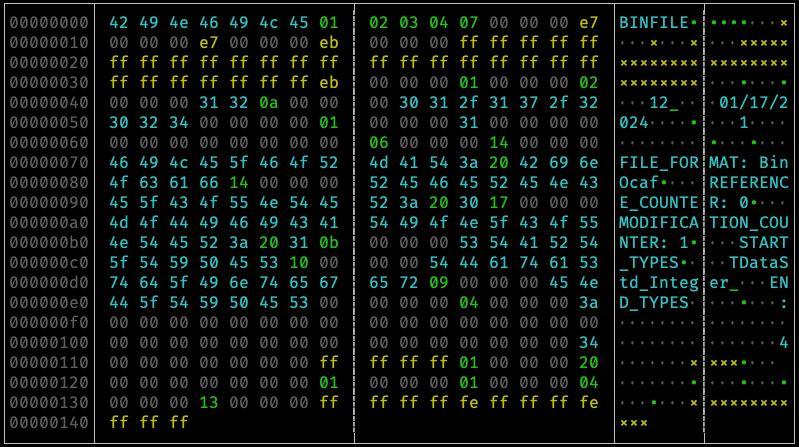
\includegraphics[width=.9\linewidth]{./img/binocaf-binary-content.png}
\end{center}

我们可以大致看到文档中包含了 creation-date file-format, reference-counter, modification-counter, \texttt{TDataStd\_Integer} 等一些信息。
\subsection{相关的 OCCT 类}
\label{sec:org335a9f0}

\subsubsection{\texttt{TDocStd\_Application} class}
\label{sec:orga165cec}

类 \texttt{TDocStd\_Application} 用于创建、打开、保存、关闭和管理 OCAF 文档(\texttt{TDocStd\_Document}),支持多文档界面(MDI),允许同时处理多个文档。它是开发基于 OCAF 的应用程序的关键组件。

\begin{itemize}
\item \texttt{NewDocument(format: String, TDocStd\_Document\&)} 创建一个新的文档
\item \texttt{Open(path: String, TDocStd\_Document\&)} 打开磁盘上的一个文档
\item \texttt{Save(TDocStd\_Document\&)} 保存文档
\item \texttt{SaveAs(TDocStd\_Document\&, path: String)} 文档另存为
\item \texttt{Close(TDocStd\_Document\&)} 关闭文档
\end{itemize}
\subsubsection{\texttt{TDocStd\_Document} class}
\label{sec:orgd48ac12}

类 \texttt{TDocStd\_Document} 代表一个 OCAF 文档,用于存储和管理复杂的工程数据。它包含一个或多个层次化的数据结构(通过 \texttt{TDF\_Label} 组织)。OCAF 文档支持事务处理机制,提供了 Undo/Redo 接口;支持文档的保存和加载。

\begin{itemize}
\item \texttt{IsSaved()} 检查文档是否已保存
\item \texttt{IsEmpty()} 检查文档是否为空,即 main label 是否包含 attributes
\item \texttt{NewCommand()} 启动一个新的事务或命令
\item \texttt{CommitCommand()} 提交当前事务,使其更改称为文档的一部分
\item \texttt{Undo()}, \texttt{Redo()} 撤销或重做最近的事务
\item \texttt{GetUndoLimit()}, \texttt{SetUndoLimit(int)} 获取和设置撤销操作的限制
\item \texttt{IsChanged()} 检查文档子上次保存后是否被修改
\item \texttt{SetModified(TDF\_Label\&)} 标记一个 label 为 modified,文档变为 UnValid 状态
\item \texttt{Recompute()} 重新计算,传播 modification 的影响
\item \texttt{IsValid()} 检查文档修改后,是否重新计算了
\item \texttt{Main()} 获取文档的 main label
\item \texttt{DumpJson(OStream\&)} 打印文档内容,用于调试
\end{itemize}
\subsubsection{\texttt{TDF\_Label} class}
\label{sec:orgbffcc0e}

类 \texttt{TDF\_Label}
\subsubsection{\texttt{TDataStd\_Integer} class}
\label{sec:org78aeeaf}

\subsubsection{\texttt{BinDrivers} class}
\label{sec:org2b84a13}
\section{OCAF 实现参数化设计}
\label{sec:org6fd0970}

下面的代码基于 OCAF 实现了一个参数化设计程序。
\section{使用 IVtk Package 实现一个 VTK 模型查看器}
\label{sec:orgfece859}
\end{document}
